\documentclass[a4paper,12pt,oneside,openright]{report}


\usepackage[a4paper]{geometry}
\usepackage[T1]    {fontenc }% Allow accented output charachters
\usepackage[utf8]  {inputenc}% Allow accented input charachters 
\usepackage        {lmodern }% Modern output font	
\def\magyarOptions{suggestions=no}
\usepackage[magyar]{babel}	   % Set document language to use
\usepackage		 {amsmath}%Math mode additions
\usepackage		 {amsfonts}
\usepackage		 {floatrow}% Append additional information to images (source)
\usepackage		{mathtools}
\usepackage[pdftex]{graphicx}% Adds the ability to include images 
\usepackage		 {xcolor   }% Colors are fun :)
\usepackage        {colortbl}% Named even more. 
\usepackage        {url     }% Makes urls clickable 
\usepackage		{array}
\usepackage		 {tikz	  }% Latex drawn figures
\usepackage		{wrapfig}
\usetikzlibrary	 {matrix  }
\usepackage		{textcomp}
\usepackage        {scalefnt }% Scale the latex drawn figure elements
\usepackage[pdf]{pstricks}
\usepackage{subfigure}

% The csquotes should be used with bable to help with the references formating 
\usepackage[style=english]{csquotes} 
% Biblatex
\usepackage[style=ieee,
backend=biber,babel=other*, language=english, sorting=none,
backref=false]{biblatex} \DeclareSourcemap{ % Unfortunetly the
% bibtex currently knows of online type, not webpage. For now just map it.
  \maps[datatype=bibtex]{
    \map{
      \step[typesource=webpage, typetarget=online]
    }
  }
}

\newcommand*\circled[1]{\tikz[baseline=(char.base)]{
            \node[shape=circle,draw,inner sep=1pt] (char) {#1};}}

% Smiley commands
\newcommand{\smiley}{\tikz[baseline=-0.75ex,ColorGreyish]{
    \draw circle (2mm);
\node[fill,circle,inner sep=0.5pt] (left eye) at (135:0.8mm) {};
\node[fill,circle,inner sep=0.5pt] (right eye) at (45:0.8mm) {}; \draw
(-145:0.9mm) arc (-120:-60:1.5mm);
    }
}

\newcommand{\frownie}{\tikz[baseline=-0.75ex,orange]{
    \draw circle (2mm);
\node[fill,circle,inner sep=0.5pt] (left eye) at (135:0.8mm) {};
\node[fill,circle,inner sep=0.5pt] (right eye) at (45:0.8mm) {}; \draw
(-145:0.9mm) arc (120:60:1.5mm);
    }
}

\newcommand{\neutranie}{\tikz[baseline=-0.75ex,black]{
    \draw circle (2mm);
\node[fill,circle,inner sep=0.5pt] (left eye) at (135:0.8mm) {};
\node[fill,circle,inner sep=0.5pt] (right eye) at (45:0.8mm) {}; \draw
(-135:0.9mm) -- (-45:0.9mm);
    }
}
% Background highlight color used for the source code and the tables
\definecolor{bgSrc}{rgb}{0.95,0.95,0.95}

\usepackage[unicode]{hyperref}% - Add links between the doc
\usepackage[all]{hypcap}   %Let the links point above figures and not below
\usepackage[numbered,
			  open, 
			  openlevel=2,
			  atend]{bookmark}% - We want numbers

\hyphenation{MonetDB}
\hyphenation{BigTable}
\hyphenation{MapReduce}
\hyphenation{Amazon}
\begin{document}

% A címlap
% !TeX encoding = UTF-8 
% !TeX spellcheck =hu_HU
\hypersetup{pageanchor=false}
\begin{titlepage}
\newcommand{\HRule}{\rule{\linewidth}{0.5mm}}
\begin{center}


\includegraphics[width=0.5\textwidth]{./kepek/Budapest-logo.jpg}\\
\textsc{Budapest Műszaki és Gazdaságtudományi Egyetem}\\
\textsc{Villamosmérnöki és Informatikai Kar}\\
\textsc{Számítástudományi és Információelméleti Tanszék}\\[1.5cm]
\textsc{Rendszeroptimalizálás -- BMEVISZM117}\\[0.5cm]

% Title
\HRule \\[0.4cm]
{ \huge \bfseries Rendszeroptimalizálás}\\[0.4cm]
{Vizsga tételsor jegyzet}

\HRule \\[1.5cm]

% Author and supervisor
\begin{minipage}{0.4\textwidth}
\begin{flushleft} \large
\emph{Szerző:}\\
\textsc{Gábor} Bernát
\end{flushleft}
\end{minipage}

\vfill
% Bottom of the page
{\large \today}
\end{center}
\end{titlepage}
\hypersetup{pageanchor=false}


\tableofcontents
\chapter{Lineáris programozás}
\hyphenation{Egerváry}
\section{Egerváry algoritmusa, az optimális hozzárendelés problémája}

Az optimális hozzárendelés problémája a következő kérdésre keresi a választ:
hogyan rendelünk egymáshoz két halmaz elemeit valamilyen optimum kritérium
szerint? Ilyen kritériumok lehetnek a maximális párosítás~\footnote{ Párosításnak
nevezünk egy $M$ élhalmazt, ha semelyik két élnek nincs közös pontja (független
él halmaz). Egy párosítás teljes, ha a gráf minden pontját lefedi.}, minimális
idő igény és így tovább. Grafikusan ábrázolva, legyen:

\begin{figure}[ht]
\caption{Egy optimális hozzárendelés probléma}
\label{fig:OptHozProb}
\centering \begin{tikzpicture}[scale=1.7]
  \tikzset{ p/.style={circle,yellow,fill=red,inner sep=0pt,minimum size=0.15cm},
  }
 % the two sets
  \draw (0,0) ellipse (1.2cm and 0.3cm) node [right=2.1cm] {Elvégezendő munka -- $A$};
  \draw (0,1.5) ellipse (1.2cm and 0.3cm) node [right=2.1cm] {Rendelkezésre álló munkások --
  $B$};
  % the dots
  \node[p] (lB) at (-1, 0) {};
  \node[p] (lT) at (+1, 0) {}; 
  \node[p] (lC) at ( 0  , 0) {};
  
  \node[p] (rB) at (-1, 1.5) {}; 
  \node[p] (rT) at (+1, 1.5) {}; 
  \node[p] (rC) at ( 0, 1.5) {};
  
  % the connection between the dots
  \draw[-] (lT) -- (rC); 
  \draw[-] (lC) -- (rC); 
  \draw[-] (lB) -- (rB);
  \draw[-] (lB) -- (rT);
\end{tikzpicture} 
\end{figure}

Gráf alakban megfogalmazva, adott $G=(V, E)$ gráf, ahol $V=(A, B)$ és $E=(x,y)$,
ahol $x \in A$ és $ y \in B$. Megkülönböztetünk $3$ fajta helyzetet:
\begin{description}
  \item[Maximális párosítás problémája] Ekkor azt szeretnénk, hogy a párosítások
  száma minél nagyobb legyen.
  \item[Maximális súlyú párosítás problémája] Itt létezik minden párosításnak
  egy jósági tényezője, egy súlya: $w:E\rightarrow\mathbb{R}$; egy adott $M$
  párosítás esetén $(M\subset E)$ keressük azt, amely maximális összeget ad:
  $\mbox{max}\left\{\sum_{e\in M}{w(e)}\right\}$.
  \item[Maximális teljes párosítás problémája] Most olyan párosítás halmazt
  keressünk, amely a lehető legtöbb párosítást létrehoz, a lehető legnagyobb
  összeggel. A teljes párositáshoz szükséges, hogy a vizsgált ponthalmaz páros
  legyen. Azt, hogy ez nem ekvivalens a korábbi feladattal
  \aref{fig:OptMaxNemEkv} ábra szemlélteti. Ekkor a maximális súlyú párosítást
  az $a_2-b_1$ adja, míg a maximális teljes párosítás problémájára a helyes
  válasz az $a_1-b_1$ és $a_2-b_2$ él párok.
\end{description}

\begin{figure}[htb]
\caption{Maximális súlyú és teljes párosítás probléma}
\label{fig:OptMaxNemEkv}
\centering
\begin{tikzpicture}[scale=1.7]
  \tikzset{
  p/.style={circle,white,fill=gray,inner sep=0pt,minimum size=0.15cm},
  }
  % the dots
  \node[p] (a1) at (0, 0) {$a_1$};
  \node[p] (a2) at (1,  0) {$a_2$};
    
  \node[p] (b1) at (0, 1) {$b_1$};
  \node[p] (b2) at (1,  1) {$b_2$};
    
  % the connection between the dots
  \draw[-] (a2) -- (b1) node [midway, right] {$3$};
  \draw[-,style=dashed] (a1) -- (b1) node [near start, left] {$1$};
  \draw[-,style=dashed] (a2) -- (b2) node [near start, right] {$1$};
\end{tikzpicture} 
\end{figure}

A maximális súlyú párosítás problémája \emph{visszavezethető} a maximális tejles
súlyú párosítás problémájára. A transzformációhoz a kevesebb csúcsú halmazt ($A$
és $B$ közül) egészítsük ki, hogy a két halmaz számossága megegyezen. Majd a
hiányzó és negatív súlyú éleken (a két halmazt közt) legyen $w=0$. 

\subsection{Magyar módszer}

Megoldás ad a maximális párosítás problémára polinomiális időben. Induljunk ki
bármilyen meglévő párositásból, egy ilyent \aref{fig:MagyModHelyeseg} ábra mutat
be.

\colorlet{ColorPink}{red!10}
\colorlet{ColorBlue}{blue!20}

\begin{figure}[htbp]
\caption{Magyar módszer helyessége}
\label{fig:MagyModHelyeseg}
\centering
\begin{tikzpicture}[font=\small,scale=1.7]
  \tikzset{
  p/.style={circle,white,fill=gray,inner sep=0pt,minimum size=0.15cm},
  }
  % the dots
  \draw[fill,ColorPink] (0.5,0) ellipse (0.7cm and 0.2cm) node [above=10pt,black] {$B_3$};
  \node[p] (B31) at (0,  0) {};
  \node[p] (B32) at (1,  0) {};
  
  \draw[fill,ColorBlue] (4,0) ellipse (1.5cm and 0.2cm) node [above=10pt,black] {$B_2$};
  \node[p] (B21) at (3,  0) {};
  \node[p] (B22) at (4,  0) {};
  \node[p] (B23) at (5,  0) {};
  
  \draw[fill,ColorPink] (7,0) ellipse (0.35cm and 0.2cm) node [above=10pt,black] {$B_1$};
  \node[p] (B11) at (7,  0) {};
  
  \node[p] (A31) at (0,  -1) {};
  \node[p] (A32) at (1,  -1) {};
  \draw (0.5,-1) ellipse (0.7cm and 0.2cm) node [below=10pt] {$A_3$};
  
  \draw[fill,lightgray] (4,-1) ellipse (1.5cm and 0.2cm) node [below=10pt,black] {$A_2$};
  \node[p] (A21) at (3,  -1) {};
  \node[p] (A22) at (4,  -1) {};
  \node[p] (A23) at (5,  -1) {};
  
  \draw[fill,lightgray] (7.5,-1) ellipse (0.7cm and 0.2cm) node [below=10pt,black] {$A_1$};
  \node[p] (A11) at (7,  -1) {};
  \node[p] (A12) at (8,  -1) {};
    
  \draw[-, color=blue, style=dashed] (A32) -- (B11);
  \draw[-, color=black, thick] (A31) -- (B31);
  \draw[-, color=black, thick] (A32) -- (B32);
  
  \draw[-, color=black, thick] (A21) -- (B21);
  \draw[-, color=black, thick] (A22) -- (B22);
  \draw[-, color=black, thick] (A23) -- (B23);
  
  \draw[-, color=ColorGreyish, thick] (A31) -- (B21);
  \draw[-, color=ColorGreyish, thick] (A32) -- (B31);
  \draw[-, color=ColorGreyish, thick] (A22) -- (B21);
  \draw[-, color=ColorGreyish, thick] (A22) -- (B23);
  
  \draw[-, color=ColorGreyish, thick] (B22) -- (A11);
  \draw[-, color=ColorGreyish, thick] (B23) -- (A12);
  
\end{tikzpicture} 
\end{figure} 

Egy ilyen gráfon végezzük el a következő definiciókat: 

\begin{description}
  \item[Alternáló út] olyan él sorozat (séta) amely $A$-ból indul és minden második 
  él párosításbeli.
  \item[Javító út] olyan alternáló út amely $B$-ben végződik.  
\end{description}

Ekkor a magyar módszer algoritmus lépései:

\begin{enumerate}
  \item Keresünk egy javító utat.
  \item Cseréljük meg az út menetén a szerepeket:
  	\begin{itemize}
  	\item párosításbeli élek kivétele,
  	\item nem párosításbeli élek betétele. 
	\end{itemize}
  \item Lépjünk, vissza az első lépéshez ameddig létezik javító út.
\end{enumerate}

Az algoritmus helyességének belátásához térjünk vissza \aref{fig:MagyModHelyeseg} ábrához,
amely egy köztes állapotot szemléltet. Legyen:
\begin{description}
  \item[$(A_1)$] -- azon csúcsok halmaza, amelyet az $M$ párosítás le nem fedett.
  \item[$(B_2)$] -- $A_1$--ből alternáló úton elérhető csúcsok halmaza,
  \item[$(A_2)$] -- $B_2$--hőz tartozó párosítás, 
\end{description}

Amennyiben az algoritmus leállt $B_2$ halmaz csúcsainak végpontja $A_2$ és $A_1$
halmazból induló élek, azaz $B_2$ lefogó pontja~\footnote{A lefogó ponthalmaz egy
adott G (rész)gráf minden élének legalább egyik végpontját tartalmazza.} az $A_1
\cup A_2$ halmaznak. Azaz elmondható, hogy $A_3$ és $B_2$ lefogó pontja a
gráfnak, ugyanakkor $A_3$ és $B_2$ elem--száma megegyezik a párosítás számával.
A \emph{König tétel}~\footnote{ A tétel Kőnig Dénestől származik. Legyen egy $G$
páros gráf, ekkor $\nu(G)=\tau(G)$ (azaz a legnagyobb független él halmaznak
ugyanannyi eleme van, mint a legkisebb lefogó pont halmaznak) és ha $G$--ben
nincs izolált pont akkor $\rho(G)=\alpha(G)$ (azaz a legkisebb lefogó él halmaz
azonos méretű a legnagyobb független pont halmazzal).} értelmében ezért a
párosítás maximális.

\subsection{Egerváry algoritmusa}

Az Egerváry~\footnote{Egerváry Jenő} algoritmus súlyozott páros gráfokra megadja
a maximális összsúlyú teljes párosítást. Ehhez az algoritmus először definiálja
a címkézés műveletet: minden csúcshoz rendel egy valós értéket ($c:V \rightarrow
\mathbb{R}$) úgy, hogy minden él pár esetén ($\forall \left\{x,y\right\} \in E |
x \in A, y \in B$) igaz a következő kifejezés: $c(x)+c(y)>=w(e)$. Amennyiben
$c(x)+c(y)=w(e)$ legyen az él ,,piros.'' E címkézés mellet: $\sum_Mw(e) \leq
\sum_Vc(v)$, azaz a maximális összsúlyú teljes párosítás összsúlya kisebb, mint
a címkézés ősszege.

Bizonyítás, adódik a definicióból:

\begin{displaymath}
\sum_M{w} \leq \sum_M{\left[c(x)+c(y)\right]} = \sum_V{c(v)}
\end{displaymath}

\emph{Lemma}: Ha $M$--ben $\forall$ él piros, a párosítás maximális.

\subsection{Az algoritmus}

Vegyük továbbra is \aref{fig:MagyModHelyeseg} ábrát és az ott megfogalmazott definiciókat:

\begin{enumerate}
  \setcounter{enumi}{-1}
  \item lépés (inicializálás):   \begin{displaymath}
  c(v)=\begin{cases}
  \mbox{max}(w) & v \in A, \\
  0             & v \in B.
  \end{cases} 
  \end{displaymath}
  \item lépés: keressük meg a maximális elem--számú párosítást a piros részgráfban
  javító utakkal.
  Legyen ez a párosítás $M'$. Ha ez maximális megállunk.
  \item lépesben legyen:
  \begin{displaymath}
  \begin{rcases}
  x \in A_1 \cup A_2, \\
  y \in B_1 \cup B_3\\
  \{x,y\} \in E
  \end{rcases}
  \Rightarrow \sigma= min\left\{c(x) + c(y) + w(\left\{x,y\right\}) \right\},
  \end{displaymath}
  Majd: \begin{displaymath}
  c'(v)=\begin{cases}
  c(v)-\sigma & v \in A_1 \cup A_2, \\
  c(v)+\sigma & v \in B_2, \\
  c(v) 		   &  \mbox{másképp.}
  \end{cases} 
  \end{displaymath}
  Végül legyen $M=M'$ és $c=c'$ és folytassuk az első lépéstől.
\end{enumerate} 

Az algoritmus helyességének alátámasztásához be kell látnunk, hogy:

\begin{enumerate}
  \item A nulladik lépés címkézés.
  \item Létezik $\left\{x,y\right\}$ a második lépésben. Ez igaz, mert ha nem
  lenne akkor $A_1 \cup A_2$ bármely szomszédja $B_2$--ben volna és a
  \emph{Hall--feltétel} \footnote{$ \forall~x_0 \subseteq A$--ra az $|N(x_0)|
  \geq |x_0|$ egyenlőtlenségnek teljesülnie kell, másképp nem létezik párosítás
  ($N~x_0$ szomszédinak halmazát fedi).} alapján nem létezne párosítás.
  \item $c'$ címkézés e? Ehhez figyeljük meg, hogy $\sigma$ hogyan változhat:
  
  \begin{tabular}{ l |  c c }
                  & $A_1 \cup A_2$ & $A_3$ \\
                  \hline
  $B_2$           & $0$            & $+\sigma$ \\
  $B_1 \cup B_3$ & $-\sigma$      & $0$ \\
  \end{tabular}
  
  Ugyanakkor a $\sigma > 0 $, hiszen $A_1 \cup A_2$ és $B_1 \cup B_3$ között
  vezető élek között nem lehet piros él. Tehát a címkézés csak egy helyt csökken
  (ami elronthatná a címkézést), de itt csak a maximális csökkenthető értékkel
  csökken, tehát a címkézés tulajdonsága megmarad.
 
  \item Ahol $\sigma$ minimális ott egy piros él keletkezik, ezáltal a piros
  részgráf is megváltozik. Ha az $\in B_1$ nő a párosítás mérete, mivel ha a
  párja $A_1$--ben van akkor simán összeköthető, ha meg $A2$--ben akkor az
  $A_1-B_2-A_2-B_1$ utón elérhető és ez hosszab mint az eredeti. 
  
  Ellenben, ha a piros él $B_3$--beli akkor $A_3$ és $B_2$ között megszűnik egy
  piros él, de ez nem befolyásolja a párositást, hiszen az új piros és $B_3$
  --beli végpontja elérhető lesz alternáló úton, ezért átkerül az $B_2$--be.
  
  Tehát $B_3$ legfeljebb $n$ lépésből elfogy. A  következő lépésben $B_1$--belli
  a piros él, tehát nő a párosítás $\Rightarrow n^2$ iterációba legfeljebb
  megvagyunk. Egy iteráció időigénye $O(e)$ (a $\sigma$ kiszámolása és $A_1 \cup
  A_2$ előállitása), tehát az algoritmus komplexitása $O(n^2e)$.
  \end{enumerate}
\newpage
\section{A lineáris programozás alapfeladata, kétváltozós grafikus megoldás és Fourier-Motzkin elimináció}

Egy egyenlőtlenségrendszer megoldásai közül kiválasztani azt, amely valamilyen
célfüggvény szerint optimális:

\begin{displaymath}
max(cx: Ax \leq b).
\end{displaymath}

Az elemek méretei: 

\begin{displaymath}
\begin{bmatrix} 1 &  \cdots &  n \end{bmatrix}
\begin{bmatrix} 1 \\ \vdots \\  n \end{bmatrix}
:
\begin{bmatrix} 1 & \cdots & n \\ \vdots & \ddots & \vdots \\ m  & \cdots & 0 \end{bmatrix}
\begin{bmatrix} 1 \\ \vdots \\  n \end{bmatrix}
\leq
\begin{bmatrix} 1 \\ \vdots \\  m \end{bmatrix}.
\end{displaymath}

Ha az egyenletnek, vagy a feladat más alakban van megadva átalakítható az
következő összefűggések alapján:
\begin{align*}
\alpha x \geq \beta  \Rightarrow  &-\alpha x \leq -\beta \\
\alpha x  =    \beta \Rightarrow  & \begin{cases}
-\alpha x \leq-\beta \\
+\alpha x \leq+\beta \\
\end{cases}\\ 
min(cx:Ax \leq b)	 \Rightarrow    & max((-c)x:Ax \leq b)
\end{align*}

A minimumos egyenlet megoldása a maximum egyenlet megoldásának az ellentéte
lesz. Ha olyan egyenletünk van, ahol szigorú egyenlőtlenség van ( $<$ vagy $>$)
akkor ezeket elhagyjuk, mert a valós számok halmazán nem tudunk hipersik közeli
értéket keresni. A kérdés amire keressük a válaszokat:

\begin{itemize}
  \item Létezik e $Ax \leq b$ egyenletnek megoldása?
  \item $cx$ korlátos e a megoldás halmazon?
  \item Melyik $x$--re maximális a $cx$ kifejezés?
\end{itemize}

\subsection{Kétváltozós feladat grafikus megoldása}

$\alpha x \leq \beta$ egyenlet meghatároz egy félsíkot, amelyet $\alpha x = \beta$
határol. Ha a félsíkok metszete véges, egy konvex sokszöget alkotnak, amely megadja a
megoldás halmazt.

\begin{figure}[htbp]
\centering
\subfigure{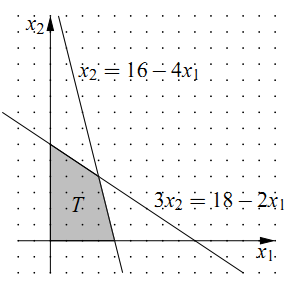
\includegraphics[height=6cm]{./kepek/2valtozo_megoldas_rajz.png}
\quad 
\subfigure{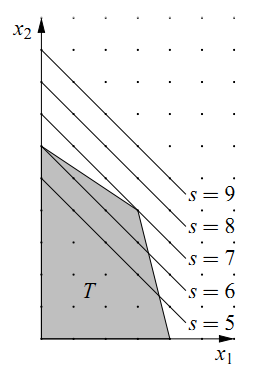
\includegraphics[height=6cm]{./kepek/2valtozo_megoldas_terulet.png} }}
\caption{Kétváltozós feladat grafikus megoldása} \label{fig:KetValtGraf}
\end{figure}

Ha a célfüggvényt különböző $x$--re felrajzoljuk meghatározható az optimális
megoldás és az ehhez tartozó $x$ értékek. Egy alternativ megkőzelités, hogy
vesszük célfügvény irányvektor normálját és ennek irányából pásztázunk végig a
meghatározott konvex sokszögben, a metszőpontok mentén. A megoldást az utolsó
megvizsgált metszőpont adja.

\subsection{Fourier-Motzkin elimináció}

Ennek segítségével megvizsgálhatjuk az egyenlet megoldhatóságát: $n$ változós
egyenletet visszavezetjük $n-1$ változóra, iteratívan, amíg egy változós
egyenletrendszert nem kapunk; erre könnyű megoldhatóságot vizsgálni. A folyamat:

\begin{enumerate}
  \item Minden egyenlet $\alpha \in \mathbb{R}^+$ szorzással az alábbi alakra
  hozható:
  \begin{displaymath}
  \begin{bmatrix}
  1  & A_+ \\
  -1 & A_- \\
  0  & A_0
  \end{bmatrix}
  \begin{bmatrix}
  x_1 & 
  x'
  \end{bmatrix}
  \leq
  \begin{bmatrix}
  b_+ \\
  b_- \\
  b_0
  \end{bmatrix}.
  \end{displaymath}
  \item 
  \begin{itemize}
  	\item Ha $A_-$ üres ($=\emptyset$): 
  	\begin{align*}
  	1 \cdot x_1 + A_+ x'     &\leq b_+ \\
  	1 \cdot x_1 + \alpha x' &\leq \beta \\
  	x_1 			  &\leq \beta - \alpha x' 
  	\end{align*} 
    Ekkor válasszuk úgy $x_1$--t, olyan kicsire hogy az összes sora e feltétel
    teljesüljön. Ezután $A_+$ teljes sorai elhagyható, továbbá elég $A_0$
    sorait vizsgálni, elhagyva a baloldalon található nulla oszlopot ($n-1$
    változós eset).
  	
  	\item Ha $A_+$ üres ($=\emptyset$): 
  	\begin{align*}
  	-1 \cdot x_1 + \alpha x'     &\leq \beta \\
  	x_1 			  &\geq \alpha x' - \beta 
  	\end{align*} 
  	Ekkor válasszuk úgy $x_1$--t, olyan nagyra hogy e feltétel teljesüljön.
  	Ezután $A_-$ elhagyható.
  	\item Ha $A_- \neq \emptyset$ és $A_+ \neq \emptyset$ akkor legyen 
  	$i \in A_-$ egy sora, $j \in A_+$ egy sora, és képezzük az összes sora az
  	alábbi ősszeget (ez exponenciális egyenlet szaporodást jelent, e miatt az algoritmus
  	futási ideje is exponenciális):
  	\[
  	\left( \alpha_i + \alpha_j \right) \cdot x' \leq b_i + b_j 
  	\]
  	Ezzel visszavezettük a kérdést $n-1$ változós estre.
  \end{itemize}
 \item Ha $n=1$ és 
 \begin{align*}
 \exists~b_0 < 0 &\Rightarrow \mbox{nem megoldható} \\
 \not \exists~A_+ \mbox{ vagy} \not \exists~A_- < 0 &\Rightarrow \mbox{megoldható} \\
 \mbox{másképp igaz, hogy } x_1 \leq \beta_+ \mbox{ és } y_1 \geq \beta_-
 &\Rightarrow \mbox{megoldható ha } \mbox{max}(-\beta_-) \leq min(\beta_+)
 \end{align*} 
  Ha $n \geq 1$ folytassuk a $2$--es lépéstől.
\end{enumerate} 

A Gauss eliminációval szemben itt csak pozítiv skalárral szorozhatjuk be a sort,
az egyenlőtlenség miatt.
\newpage
\section{Farkas-lemma (két alakban). A lineáris program célfüggvény korlátossága.}

A következő egyenletekből csak a jobb vagy csak a bal egyenletrendszereknek
létezik egy időben megoldása:

\begin{enumerate}
  \item alak: \begin{align*}
  \overbrace{Ax \leq b}^{A1}  && \overbrace{yA= 0}^{A2}\\
   			 && y\geq 0 \\
             && yb\leq 0
  \end{align*}
  \item alak:\begin{align*}
  \overbrace{Ax = b }^{B1}   && \overbrace{yA \geq 0}^{B2}\\
  x \geq 0 && yb \leq 0 
  \end{align*}
\end{enumerate}

Legyen az alábbi mérettel rendelkező mátrixok:
\[
\overbrace{\begin{bmatrix} 1 &  \cdots &  n \end{bmatrix}}^{\hbox{y}} 
\overbrace{\begin{bmatrix} 1 & \cdots & n \\ \vdots & \ddots & \vdots \\ m  & \cdots & 0 \end{bmatrix}}^{\hbox{A}}
\underbrace{\begin{bmatrix} 1 \\ \vdots \\  n \end{bmatrix}}_{\hbox{x}}
\overbrace{\begin{bmatrix} 1 \\ \vdots \\  m \end{bmatrix}}^{\hbox{b}}.
\]

\subsection{1--es alak}
Az első alak két egyenletrendszere nem megoldható egy időben mert:
\[ 0 = 0x = (yA) \cdot x = y(Ax) \leq yb.\] E utolsó egyenlőtlenség nem
egyértelmű, ellenőrizni kell, hogy:
\[ Ax \leq b \Rightarrow y(Ax) \leq (yb).\] Szerencsére ez igaz lesz a mátrix
szorzás disztributív tulajdonsága miatt. Majd tovább futatva a korábbi
gondolatunkat $yb<0$ amely ellentmond a kiinduló feltételeknek.

Definiáljuk a következő $C$ halmazt, amely egy sorvektorok halmaza:
\[ C= \left\{ z \in \mathbb{R}^{n+1}, z = y (A|b), y \geq 0 \right\}, \].
Célunk bizonyítani, hogy létezik $C$-ben $(0, \cdots, 0 , <0)$ alakú sorvektor,
ha az egyenletrendszer nem megoldható.

A halmaz zártságára az alábbi lemmák igazak ($z_1, z_2 \in C, \lambda>0$):

\begin{itemize}
  \item $z_1+z_2 \in C$, mert $\begin{rcases}
  z_1=y_1(A|b) \\
  z_2=y_2(A|b) \end{rcases} \Rightarrow z_1+z_2=(y_1+y_2)(A|b)$ ahol $y_1+y_2 \geq 0,$
  \item $\lambda z_1 \in C$, mert $
  z=y(A|b) \Rightarrow \lambda z = \lambda y (A|b)$ ahol igaz, hogy $\lambda y \geq 0$.
\end{itemize}

$(A|b)$ sorai $\in C$ mert $y(i)=1$--el felvételt nyernek $C$--be. Most hajtsuk végre a
Fourier-Motzkin eliminációt $(A|b)$--re, úgy, hogy a nullákat nem töröljük:

\begin{displaymath}
\underbrace{
\begin{array}{|cccc|c|}
\hline
 &  &  &  & \\
 &  & &  & \\
A &  & &  &b \\
 &  & & &\\
\hline
\end{array}}_{\mbox{sorai } \in~C}
\Rightarrow
\underbrace{
\begin{array}{|c|ccc|c|}
\hline
0 &  &  &  & \\
\hline
0 &  & &  & \\
0 &  & &  & \\
\hline
0 &  & & &\\
\hline
\end{array}}_{\mbox{sorai } \in~C}
\Rightarrow
\underbrace{
\begin{array}{|ccc|c|c|}
\hline
0 &  0 &0  & +1  & b_+\\
\hline
0 &  0& 0&  -1& b_-\\
\hline
0 &  0& 0& 0& b_0\\
\hline
\end{array}}_{\mbox{sorai } \in~C}
\end{displaymath}

A zártsági lemma miatt az elimináció során a mátrix sorai $C$ halmazon belül
maradnak. Továbbá ha a feladat eredetileg nem megoldható a végén sem lesz az, ez 
meg két féle képen történhet meg:

\begin{itemize}
  \item Létezik $0 \cdot x_n \leq gamma$ egyenlet, ahol $\gamma < 0$. Ennek alakja 
  $(0,0, \cdots, 0, <0),$ tehát a sor $\in C$.
  \item $\begin{rcases}
  +1 \cdot x_n \leq \alpha_i \\ 
  -1 \cdot x_n \leq \alpha_j \\
  \end{rcases} \Rightarrow  \mbox{ ellentmondáshoz meg akkor jutunk ha }
  \alpha_i < -\alpha_j.$
  
  Az $i$ sor alakja $(0, \cdots, 0, +1, \alpha_i)$, a $j$ sor meg $(0, \cdots,
  0, -1, \alpha_j)$. Ennek az összege meg $(0, \cdots, 0, 0, \alpha_i+\alpha_j)$
  ami szintén $\in C$, mivel $\alpha_i+\alpha_j<0$.
\end{itemize}

\subsection{2--es alak}

Az, hogy a két egyenletrendszer ($B1$ és $B2$) közül csak az egyik megoldható
egy időben indirekt bizonyítjuk. Legyen $x,y$ egy--egy megoldás:

\[ 0 \leq \underbrace{
		   \underbrace{(yA)}_{\mbox{sorvektor}}x = 
		  y\underbrace{(Ax)}_{\mbox{oszlopvektor}}}
		  _{\mbox{nem triviális lépés}}=yb<0\] ahol ellentmondáshoz jutunk.



Az hogy ha az egyik nem megoldható a másik igen visszavezetéssel bizonyítjuk az
$1$--es alakra. Ehhez először is kibontjuk a $B1$ alakot:
\begin{displaymath}
\underbrace{
\begin{array}{|c|c|c|}
\hline
y_1 & y_2  & y_3\\
\hline
\end{array}}_{y'}
\underbrace{
\begin{array}{|c|}
\hline
A \\
\hline
-A\\
\hline
-I \\
\hline
\end{array}}_{A'}
\leq
\underbrace{
\begin{array}{|c|}
\hline
b \\
\hline
-b\\
\hline
0 \\
\hline
\end{array}}_{b'}
\end{displaymath}

Azt állítjuk, hogy ha ez nem megoldható, akkor a $ yA \geq 0$, $yb \leq 0$ páros
igen.

\begin{align*}
\exists~y' &> 0 \\
y_1 A + y_2 (-A) + y_3(-I) &= 0 \\
y_1 \cdot b - y_2 \cdot b + y_3 \cdot 0 &<0
\end{align*}

Tehát:
\begin{align*}
(y_1 - y_2) \cdot A &= y_3 \\
(y_1 - y_2) \cdot B &< 0.
\end{align*}

Ekkor legyen $y=y_1-y_2$ és ezzel megkaptuk a $B2$ alakot, azaz igaz, hogy ez
megoldható.

\subsection{Korlátosság}

Az alábbi három kijelentés ekvivalens:

\begin{enumerate}
  \item $cx$ felülről korlátos az $Ax \leq b$ megoldás halmazon.
  \item $\not \exists$ megoldása az $ \begin{cases}
  Az \leq 0 \\
  cz > 0
  \end{cases} $ egyenletrendszernek.
  \item ~$\exists$ megoldása a~~$\begin{cases}
  yA=c \\
  y \geq 0
  \end{cases}$ egyenletrendszernek.
\end{enumerate}

A tétel bizonyítását \aref{fig:KorBizKor} ábra szerint fogjuk belátni.
 
\begin{figure}[htbp]
\caption{A korlátosság bizonyítási kőrre}
\label{fig:KorBizKor}
\centering \begin{tikzpicture}[scale=1.7]
  \tikzset{ p/.style={circle,white,fill=gray,inner sep=0pt,minimum size=0.3cm},
  }
  \node[p] (1) at (0, 0) {1};
  \node[p] (2) at (-1.5, -1) {2}; 
  \node[p] (3) at (+1.5 , -1) {3};
  
  % the connection between the dots
  \draw[-latex] (1) -- (2) node [midway, above=2pt] {($\star$)}; 
  \draw[-latex] (3) -- (1) node [midway, above=2pt] {($\cdot$)}; 
  \draw[-latex] (2) -- (3) node [midway, below] {Farkas lemma $A^T,c^T$--re};
  \draw[-latex] (3) -- (2);
\end{tikzpicture} 
\end{figure}

\newcommand*\circled[1]{\tikz[baseline=(char.base)]{
            \node[shape=circle,draw,inner sep=1pt] (char) {#1};}}
            
\begin{description}
  \item[($\star$) -- \circled{1} $\Rightarrow$ \circled{2}:]  Legyen $x_0$
  megoldása az $Ax \leq b$--nek és tegyük fel, hogy mégis létezik megoldása
  \circled{2}--nek. Ekkor legyen $\lambda > 0$, $x_0 + \lambda z$ is megoldása
  az $Ax \leq b$--nek, mert:
  \[ A(x_0+ \lambda z) = Ax_0 + \lambda (Az) \leq A x_0 + 0 \leq b \] Továbbá
  $c(x_0 + \lambda z ) = c x_0 + \lambda (cz)$, és mivel $cz>0$ a $\lambda$
  alkalmas megválasztásával ez tetszőleges nagyá tehető. Ez meg ellentmond
  \circled{1}--nek, tehát feltevésünk hamis volt.
  \item[($\cdot$) -- \circled{3} $\Rightarrow$ \circled{1}:]  Legyen egy $y$
  ami teljesíti \circled{3}--at és $x$ ami megoldása \circled{1}--nek. 
  \[ cx = (yA)x = y(Ax) \leq yb \]
  Ekkor $yb$ felső korlát az $Ax$ megoldás halmazán $cx-re$, tehát \circled{3}--ból
  következik \circled{1}.
\end{description}

\skiptooddpage 
\section[A lineáris programozás dualitás tétele]{A lineáris programozás dualitás
tétele (két alakban), a lineáris programozás alapfeladatának bonyolultsága}

\subsection{A lineáris programozás dualitás tétele (két alakban)}
A tétel kijelenti, hogy ha: 

$ \begin{rcases}
\mbox{LP: max}\left\{cx:Ax \leq b\right\} \\
\mbox{megoldható} \\
\mbox{felülről korlátos}
\end{rcases} \Rightarrow$ $\begin{cases}
\circled{1} \begin{cases}
\mbox{DP: min} \left\{ yb:yA = c, y \geq 0 \right\} \\
	\mbox{megoldható} \\ 
	\mbox{alulról korlátos}  
\end{cases} \\
\circled{2} \begin{cases}
\mbox{LP--nek } \exists \mbox{ maximuma} \\
\mbox{DP--nek } \exists \mbox{ minimuma} 
\end{cases}\\
\circled{3} \mbox{ maximum } = \mbox{ minimum}
\end{cases}$

Ezzel ekvivalens alakja az LP és a DP-nek a:
\begin{align*}
\mbox{LP: max} &\left\{ cx:Ax \leq b, x \geq 0 \right\} \\
\mbox{DP: min} &\left\{ yb:yA \geq c, y \geq 0 \right\}.
\end{align*}

Az \circled{1}--est bizonyítottuk az LP korlátosságánál, a \circled{2} és 
\circled{3}--hoz felhasználjuk a következő \emph{lemmát}:

\[
\begin{rcases}
Ax \leq b \mbox{ megoldható} \\
t \in \mathbb{R} \\
Ax \leq b \mbox{--nek } \not \exists~x \mbox{ megoldása, hogy } cx \geq t
\end{rcases} \Rightarrow
\parbox[t]{6cm}{
$\{yA=c, y \geq 0\}$--nak $\exists$ olyan megoldása amelyre  $yb < t$.}
\] A lemma \emph{bizonyításhoz}, átfogalmazzuk a bal oldalt mint egy Farkas
lemma alak:
$\begin{cases} Ax \leq b \\
-cx \leq -t \end{cases}$, és tudjuk, hogy a rendszer nem megoldható (nem
létezzik $x$ ami teljesiti). Alkalmazzuk rá a Farkas--lemmát, ennek második
alakja felírható, mint ($\lambda \geq 0, y
\geq 0$):
\begin{align*}
\begin{bmatrix} y & \lambda\end{bmatrix}
\begin{bmatrix} A \\ -c \end{bmatrix} = yA - \lambda c = 0 &\Rightarrow 
yA = \lambda c, \\
\begin{bmatrix} y & \lambda\end{bmatrix}
\begin{bmatrix} b \\ -t \end{bmatrix} =yb~ - \lambda t < 0 &\Rightarrow 
yb < \lambda t
\end{align*}

Ha $\lambda=0 \Rightarrow \begin{rcases}
yA = 0, \\
y \geq 0, \\
yb <  0 \end{rcases} \xRightarrow{\text{Farkas--lemma}}$ $Ax \leq b$ nem
megoldható, de ez ellentmondás az állításnak, tehát $\lambda$ nem lehet nulla
($\lambda \neq 0$). Legyen $y'=\frac{1}{\lambda}y$ így az egyenletrendszer
$y'A=c,~y'\geq0,~y'b<t$ alakú lesz és ezzel megadtunk minden $y$--ra egy
$y'$--et amely teljesíti a lemma kijelentését.

A \circled{2} \emph{bizonyításához} tegyük fel, hogy $\not \exists$ maximum
LP--n, ekkor legyen $t=\mbox{sup}\left\{cx:Ax \leq b \right\}$ (hiszen bármely
$x \subseteq R, x \neq \emptyset, x$ felülről korlátosnak $\exists$ szuprémuma,
legkisebb felső korlátja, ha még maximuma nincs is). Ha $t$ nem maximum
$\Rightarrow Ax \leq b$--nek $\not \exists~cx \geq t$--t teljesítő megoldása.
Ekkor:

\[ cx = (yA)\cdot x = y (Ax) \leq yb < t.\]

Így $yb$ egy $t$-nél kisebb felső korlát $cx$-re, de ez ellentmondás, tehát t
nem szuprémum és feltevésünk hamis volt, létezzik maximum LP--n. A DP--n történő
bizonyításhoz használjuk fel az LP bizonyítást, átírva a feladatott max--ra ($E$
-- egység mátrix):

\[ max \left\{ (-b)^T y^T :
\begin{cases}
(~~A^T)y^T    &\leq~~c^T \\
(-A^T) y^T &\leq -c^T \\
(-E~~)y^T    &\leq~~0 \\
\end{cases}  \right\} \]
 
A \circled{3} \emph{bizonyításához} már láttuk, hogy a \[ \mbox{max}\left\{
cx:Ax \leq b \right\} \leq
   \mbox{min}\left\{ yb:yA = c, y \geq 0 \right\}
\] fennáll. Legyen $t=\mbox{min}\{ yb:yA~=~c, y~\geq~0 \}$ és tegyük fel, hogy a
fenti egyenlőtlenségben nem egyenlőség áll.  Tehát ekkor az LP--nek
$\not\exists~cx \geq t$ kifejezést teljesítő megoldása, amiből következik,
hogy a duális feladatnak van olyan megoldása amire $yb<t$. De ez ellentmondás t
választásának, tehát feltevéssünk hamis volt.

\subsection{LP bonyolultság}

Az LP feladat megfogalmazható, mint eldöntési probléma: $\exists?$ az $Ax \leq
b$--t kielégítő x vektor amelyre $cx\geq t$? A probléma NP--beli. Tanú egy ilyen
$x$. Ugyanakkor coNP--beli is, a duális feladat megoldása tanú erre. $x, y$
mérete véges.

\begin{description}
  \item[1947 -- Dantzig -- Szimplex módszer] Hatékony gyakorlati feladatokon, de
  exponenciális komplexitású.
  \item[1979 --  Hacsijan -- ellipszoid módszer] Polinomiális komplexitás, de
  gyakorlatban lassú.
  \item[1984 --  Karmakar -- belső pontos módszer]  Polinomiális, hatékonyabb az
  ellipszoidnál, de ez is a gyakorlatban lassabb a szimplexnél.
\end{description}
\newpage
\section{Egészértékű programozás: a feladat bonyolultsága, korlátozás és szétválasztás (Branch and Bound)}

\subsection{Egészértékű programozás}
A feladat:
\begin{align*}
IP &: \mbox{max }{cx: Ax \leq b, x \mbox{ egész}} \\
DIP &: \mbox{min }{yb: yA=c, y \geq 0, y \mbox{ egész}}
\end{align*}
\[ \mbox{max(IP)} \leq \mbox{max(LP)}= \mbox{min(DLP)} \leq \mbox{min(DIP)} \]

A feladat bonyolultságának meghatározásához fogalmazzuk át eldöntési problémára:
$\exists?~Ax \leq b,~ x$ egész között olyan vektor, amelyre $cx \geq t?$ Az IP
feladat NP--teljes. NP--beli mert x tanú. A dualitás tétel nem alkalmazható
mivel max(IP)~$<$~min(DIP) fent állhat, tehát a probléma nem coNP--beli. \emph{NP
teljes}, visszavezethető a $3$--SAT problémára.

A bizonyításhoz megadjuk a visszavezetést: definiálunk egy eljárást, amely tetszőleges
logikai függvényhez megad egy olyan IP problémát, melyre akkor és csak akkor igenlő a
válasz, ha a függvény kielégíthető. A függvény alakja:

\[ f(x_1, x_2, \cdots, x_k) = \bigwedge_{i=1}^{d}{\left( x_{i_1}^{e_{i_1}} \vee 
x_{i_2}^{e_{i_2}} \vee x_{i_3}^{e_{i_3}}\right).} 
\]
Az IP probléma ismeretlenjei legyen $z_{i=\overline{1,k}}$ egyenlőtlenségek, ahol 
$0 \leq z_{i=\overline{1,k}} \leq 1$. Továbbá minden diszjunkcióra is felírunk egy
egyenlőtlenséget:


\begin{align*}
z_{i_1} &+ z_{i_2} &+      z_{i_3}  &\geq 1 & \mbox{ ha }~~x_{i_1} \vee~~x_{i_2}\vee~~x_{i_3}& \\
z_{i_1} &+ z_{i_2} &+ (1 - z_{i_3}) &\geq 1 & \mbox{ ha }~~x_{i_1} \vee~~x_{i_2} \vee \neg x_{i_3}& \\
z_{i_1} &+ (1-z_{i_2}) &+ (1 - z_{i_3})  &\geq 1 & \mbox{ ha }~~x_{i_1} \vee \neg x_{i_2} \vee\neg x_{i_3}&\\
(1-z_{i_1}) &+ (1-z_{i_2}) &+ (1 - z_{i_3})  &\geq 1 & \mbox{ ha } \neg x_{i_1} \vee \neg x_{i_2} \vee \neg x_{i_3}&
\end{align*}

Ha $f$ kielégíthető, akkor $z_i=1 \Leftrightarrow x_i=$ ,,igaz''. Ez lesz az
egyenletrendszer egészértékű megoldása. 

Megfordítva, ha az egyenlőtlenség--rendszert egész $z_i$ értékkel ki tudjuk
elégíteni akkor -- mivel minden egész vagy $0$, vagy $1$ -- az $x_i$=,,igaz''
$\Leftrightarrow z_i=1$ választással $f$--et kielégítő értéket adtunk a logikai
változónak.

Eközben a $\sum_{i=1}^{k}{z_i}$ összeg értétek valahol $0$ és $k$ között adódik,
tehát $c=(1,1,\cdots,1)$ választással tulajdonképpen a \emph{,,Van-e az
$(1a-1b$) és a $*(2a-2d$ feltételeket kielégítő (egész) vektorok között olyan,
melyre $cx \geq 0$?''} kérdést tesszük fel. Az így kapott IP feladatra a válasz
akkor és csak akkor igenlő, ha az f kielégíthető.

\subsection{A korlátozás és szétválasztás az IP feladatra}

Alakja $\mbox{max} \left\{cx:Ax \leq b, f \leq x \leq g| x,f,g \in \mathbb{Z}^n
\right\},$ ahol az $f$ és $k$ korlátok, amelyek biztosítják, hogy a feladat véges
lépésben megoldható. A metódus kulcs gondolata, hogy az IP feladat megoldásához először
megoldjuk mint LP, ha az eredmény egész megvagyunk, egyébként tovább bontjuk két kisebb
IP feladatra. Legyen $z^*=cx^*$, az egyenlőtlenség mindig $Ax \leq b$ marad.

Az algoritmus folyamata:

\begin{enumerate}
  \setcounter{enumi}{-1}
  \item $\overbrace{L=\left\{ \left(
  \overbrace{f}^{\text{alsó}},\overbrace{g}^{\text{felső}},\overbrace{\infty}^{w
  \text{ -- maximum értéke}} \right) \right\}}^{\text{IP részfeladatok}},
  \overbrace{z^*=-\infty}^{\text{eddigi legjobb célfüggvény érték}},
  \overbrace{x^*}^{\text{legjobb megoldás}}$
  \item Ha $L=\emptyset \Rightarrow$ \emph{vége} és a megoldás az aktuális $z^*$
  és $x^*$.
  
  Egyébként $L$--ből vegyük ki IP$_i$ feladatott.
  \item Ha $w_i \leq z^*$, IP$_i$--nek a megoldása nem lehet $z*$--nál jobb,
  folytassuk az első ponttól (ez a \emph{Bound} lépés).
  \item Oldjuk meg a relaxált IP$_i$ feladatott (LP$_i$--t).
  \\ Ha $\not \exists$ megoldás visszalépünk az első ponthoz.
  \\ Egyébként: $z_i$ -- maximum érték,  $x_i$ -- maximum hely.
  \item Ha $z_i \leq z^*$, IP$_i$ feladat és rész feladatai maximum értéke is
  legfeljebb $z^*$, lépjünk vissza az első ponthoz.
  \item Ha $z_i > z^* \mbox{ és } x_i \in \mathbb{Z}^{n}$ akkor $ z^* = z_i, x^* =
  x_i$ (adat frissítés) és visszalépünk az első ponthoz.
  \item Választunk egy közbenső értéket $(f_{i_j} \leq t \leq g_{i_j})$ és egy
  ezt meghatározó $x_j$ elágazás változót $x_i$--ből ($j$ egy pozíció $x$
  vektorban, $i$ az IP feladat sorszámát jelöli). Ezután $L$--ben elhelyezzünk
  két új feladatott:  $(t+1, g, z_i)$ és $(f, t, z_i)$. Lépjünk vissza az első
  ponthoz (\emph{Branch} lépés).
\end{enumerate} 

Az algoritmus véges sok lépésben leáll és megtalálja a feladat optimumát. A
véges sok lépést $f$ és $k$ vektor garantálja, hiszen a kezdetben kitűzött
feladatnak csak véges sok rész problémája lehet a felhasznált korlátok miatt. Az
optimális részt indirekt bizonyítjuk: legyen $z_0$ az optimum, de az eljárás
$z*<z_0$--t kapta.

Állítjuk, hogy $L$--ben mindig kellet, hogy legyen olyan IP$_i$ feladat amelynek
az optimum értéke $z_0$. Ez kezdetben fent áll, és az algoritmus egy ilyen IP
feladattal a $5.$--ik vagy $6.$--ik lépéshez jut el. Ha az ötödikbe jut akkor az
algoritmus mégis csak megtalálja a $z_0$ optimumot, ami ellentmondás.

Ha a hatodik lépés következik be, akkor a két keletkező IP feladat közül az
egyikre teljesül, hogy a vizsgált tartományában a $z_0$--hoz tartozó optimum
benne van, így $z_0$ optimumot mindenképp megtaláljuk. Tehát az eljárás során a
lista sosem ürült ki, de ekkor az algoritmus sose állhatott volna le, ami a
keresett ellentmondás.

\subsection{Gyakorlati tanácsok}
\begin{itemize}
  \item LIFO alapú új feladat választás $L$--ből, mert a megoldás várhatóan
  mélyen van a fába és ez tud legmélyebbre leggyorsabban lenyúlni.
  \item Elágazásnál a legkevésbé egész $x_j$--t válasszuk elágazási változónak
  (amelynek törtrésze $\frac{1}{2}$-höz legközelebb van), közbülső értéknek
  pedig ennek egész értékét.
\end{itemize}
\newpage
\section{Totálisan unimoduláris mátrixok és alkalmazásai}

Egy totálisan unimoduláris mátrixn minden négyzetes részmátrixának determinánsa
$0, 1$ vagy $-1$. Ehhez szükséges (de nem elégséges) feltétel, hogy a mátrix
elemei is csak $0, 1$ vagy $-1$ lehetnek.

\[
\begin{rcases}
A \text{ totálisan unimoduláris -- TU} \\
b \text{ egész vektor} \\
c \text{ tetszőleges} \in \mathbb{R}^n \\
\text{max} \left\{ cx:Ax \leq b \right\} \text{ LP feladat}\\
\text{ami megoldható és véges}
\end{rcases} \Rightarrow \parbox[t]{8cm}{ Az IP feladat is megoldható és
maximuma megegyezik az IP feladat maximumával.}
\]

\emph{Lemma:} a totálisan unimoduláris tulajdonság megmarad, ha:

\begin{description}
  \item[sor vagy oszlopot $\cdot (-1)$] $\Rightarrow$ ekkor a determináns
  előjele változik meg.
  \item[egységvektor sor vagy oszlopként való hozzáadása] $\Rightarrow$ ha a
  mátrixhoz egységvektort veszünk hozzá például oszlopként, és egy kiválasztott
  négyzetes részmátrixában ez az oszlop szerepel, akkor az új oszlop szerinti
  kifejtésből azonnal látszik, hogy a determináns megegyezik az eredeti mátrix
  egy négyzetes részmátrixának determinánsával vagy annak ellentettjével, így
  értéke $0, 1$ vagy $-1$.
  \item[sor vagy oszlop ismétlés] $\Rightarrow$ ha a kiválasztott részmátrixba
  az eredeti is szerepel a determináns nulla lesz, ha csak az egyik marad, akkor
  előáll az eredeti mátrixból képzett részmátrix, amely determinánsának értéke
  megmarad $0, 1$ vagy $-1$. 
  \item[transzponáljuk] $\Rightarrow$ megmarad a determináns definiciójának
  következményeként.
\end{description}

\emph{Tétel. Bármely irányitott gráf illekszkedés mátrixa~\footnote{$ 
B(G_{(V,E)})=
b_{i_{\in V}j_{\in E}}=
\begin{cases}
0  & \text{ha a } j \text{--edik él nem illleszkedik az } i \text{--edik ponthoz,} \\
+1  & \text{ha a } j \text{--edik élnek az } i \text{--edik pont kezdőpontja,} \\
-1  & \text{ha a } j \text{--edik élnek az } i \text{--edik pont a végpontja,} \\
+1  & \text{ha a } j \text{--edik él az } i \text{--edik ponthoz illeszkedő hurokél.} \\
\end{cases}$} totálisan unimoduláris.}.\\

Irányitott illeszkedési mátrixnál az oszlopban $1$ van amely pontból indul az
él, $-1$ ahove mutat; hurokél esetébben egyetlen $1$--es található. A
bizonyitást teljes indukcióval. Legyen $M \in \mathbb{M}_{k\times k}$ méretű
részmátrix. Ha $k=1$ az állitás nyilvánvaló. Ha $k \geq 2$ és létezzik egy darab
oszlop amelybe legfeljebb egy nem nulla elem van, akkor kifejtés aszerint és az
indukció adja a többit. Másképp minden oszlopábban egy darab $+1$ és egy darab
$-1$ van. Így $M$ sorainak összege nullvektor $\Rightarrow$ det$M=0$.\\

\emph{Tétel. Páros gráf~\footnote{Páros gráfnak nevezünk egy $G$ gráfot, ha
csúcsainak halmazát fel tudjuk úgy osztani egy $A$ és $B$ halmazra, hogy az
összes $G$-beli élre teljesül, hogy az egyik végpontja $A$-ban van, a másik
pedig $B$-ben.} illeszkedési mátrixa totálisan unimoduláris.}\\ 

Mutason minden él $A$--ból $B$--be. Irányított gráf illeszkedési mátrixe TU. Az
eredeti illeszkedési mátriszának megkapásához $B$ csúcsainak megfelelő sorokat
$-1$--el szorozzuk.

\subsection{Maximális összsulyú párositás IP feladatként}

Legyen $x$ indikátor, hogy az él benne van e párositásban, $w$ egy tetszőleges
él súlyfüggvény és $B$ az illeszkedési mátrix (amely páros gráf lévén totálisan
unimoduláris). A \emph{feladat}, megfogalmazható mint max$\left\{ wx:Bx <= (1,
\cdots, 1)^T, x \geq 0 \right\}$. Az $x \geq 0 $ feltételt bevisszük $B$
mátrixba kiegészitve azt egy $m \times m$--es egységmátrix ellentettjével, de ez
nem változtat TU tulajdonságon. 

Az egyenlőtlenség így azt fejezi ki, hogy egy csucsból legfeljebb egy kiinduló
élet választunk ki, ami adja a párositás feladatát. 

\[
\begin{rcases}
B'=\begin{bmatrix} B \\ -I \end{bmatrix} \text{ TU} \\
b \text{ egész}
\end{rcases} \Rightarrow x \text{ egész vektor ($0$ vagy $1$) értékű -- IP feladat}
\]

A max$\left\{ wx : Bx \leq (1,\cdots,1)^T, x \geq 0 \right\}$ duálisa
min$\{ y(1,\cdots,1)^T : yB \geq w,$ $y~\geq~0\}$. Az $y$ megoldás
minden $v$ csúcshoz $c(v)$ címkét rendel, ahogy Egerváry Jenő párositás
algoritmusa is:

\[ yB \geq w \Rightarrow c(a) + c(b) \geq w(e), \forall e=\{a,b\}\in E.\]

\subsection{Intervallumgráf}

A számegyenes véges sok intervallum alkossa egy gráf csúcshalmazát, és két csúcs
akkor legyen szomszédos, ha a megfelelő intervallumok metszők; az így
meghatározott gráf az intervallumgráf. Felthető, hogy a gráfot meghatározó
intervallumok $n$--re az $[1,n]$ egész végpontú, zárt részintervallumai.

Legyen az $I=\left\{I_1, I_2, \cdots, I_n\right\}$ intervallumrendszer.
Rendeljük ehhez $n \times m$--es $A(I)$ mátrixot: sorai feleljenek meg az
$1,2,\cdots,n$ egészeknek, oszlopai peddig az I intervallumainak. Az $i$--ik sor
és a $j$--ik oszlop kereszteződésben akkor álljon $1$--es, ha $i \in I_j$, és
minden más helyen álljon $0$. \\

\emph{Tétel. Az így definiált A(I) mátrix totálisan unimoduláris.} \\

A bizonyitáshoz kiválasztunk egy tetszőleges $k \times k$ részmátrixot, majd
teljes indukciót használunk az egyesek darabszáma szerint. Ha nulla darab
egyesből áll a mátrix az nyilván TU. Ha ven benne két oszlop amelyben az első
egyes azonos helyen áll, akkor a nagyobb egyes darabszámúból kivonjuk a kisedd
darabszámot. Ez az egyesek darabszámát csökkenti, de a detereminását nem
változtatja.

Ha nincs ilyen szolop, de van csupa null oszlop, akkor a determináns nulla. Ha
egyik sem teljesül, akkor pedig be tudjuk rendezni az oszlopkat úgy, hogy az
alsó háromszögmátrixot kapunk oszlop cserével. Ez a művelet a determinánst csak
előjelbe változtatja meg, így a determináns egy vagy minusz egy marad. \\

\emph{Tétel. Az intervallumgráfok tetszőleges k színre megszinezhetőek
egyenletesen.}\\ 

Az egyenletesen alatt azt értjük, hogy ha $i$--t tartalmazó intervallumok száma
$d_i$, akkor ezek közül minden felhasznált szín esetén az ilyen szinű
intervallumok száma $\lceil \frac{d_i}{k} \rceil$~\footnote{felső egészrész}
vagy $\lfloor \frac{d_i}{k} \rfloor$~\footnote{alsó egészrész}.

Elég bebizonyitani, hogy az intervallumok közül kiválasztható néhány úgy, hogy
az intervallum közül kiválasztható néhány úgy, hogy bármely $1 \leq i \leq n$
esetén az $i$--t tartalmazó intervallumgráfok között $\lceil \frac{d_i}{k}
\rceil$ vagy $\lfloor \frac{d_i}{k} \rfloor$ darab kiválasztott legyen. Ekkor a
kiválasztott intervallumokat megszínezzük egy szsínnel majd elhagyuk őket, a
megmaradt intervalumra meg ugyanaz $k-1$--el.

Legyen:
\[\begin{rcases}
A=A(I) \\
d = n \text{ dimenziós vektor } i \text{--ik komponense } d_i \\
\lceil \frac{d}{k} \rceil \text{ vektor } i \text{--ik komponense} \lceil \frac{d_i}{k} \rceil \\
\lfloor \frac{d}{k} \rfloor \text{ vektor } i \text{--ik komponense} \lfloor \frac{d_i}{k} \rfloor \\
\lfloor \frac{d}{k} \rfloor \leq Ax \leq \lceil \frac{d}{k} \rceil, 0 \leq x \leq (1,\cdots, 1)^T
\end{rcases} \parbox[t]{6cm}{Megoldás: $x=\left( \frac{1}{k}, \cdots, \frac{1}{k} \right)^T$ ahol $A$
TU $\Rightarrow \exists$ egészértékű megoldás.} 
\]

$x$--ben $0$ és $1$ közötti elemek vannak, és egy komponense oszlop öszegge
$\lceil \frac{d}{k} \rceil$ és $ \lfloor \frac{d}{k} \rfloor$ között van. Így
ezeknap az oszlopoknak megfelelő intervalumukat kiválasztva valóbban $\lceil
\frac{d_i}{k} \rceil$ vagy $ \lfloor \frac{d_i}{k} \rfloor$ illeszkedi $i$--re.
\newpage
\section{A lineáris és egészértékű programozás alkalmazása hálózati folyamproblémákra.}

\[
\begin{rcases} 
G(V,E) \mbox{ irányított gráf} \\
s,t \in V \mbox{ két kitűntet csúcs} \\
c : E \mapsto \mathbb{R}^+ \mbox{ nem negatív kapacitásfüggvény}\\
x : E \mapsto \mathbb{R}^+ \mbox{ tetszőleges függvény}\\
\rho_x(v) \mbox{ -- } v\mbox{--be belépő élek összege } x \mbox{ szerint} \\
\delta_x(v) \mbox{ -- } v\mbox{--ből kilépő élek összege } x \mbox{ szerint}
\end{rcases} \parbox[c]{6.2cm}{ 
\begin{itemize}
  \item $x$ függvény akkor \emph{folyam}, ha \\ $\forall~v~\in~V - \{s,t\}$--re: \\ $\rho_x(v)=\delta_x(v)$
  \item $x$ megengedett, ha $\forall e \in E$--re $x(e) \leq c(e)$
  \item A folyam értéke: \\ $\delta_x(s)-\rho_x(s)=\rho_x(t)-\delta_x(t)$
\end{itemize}
 }
\]

\emph{Tétel. Ford Fulkerson: A maximális folyam értéke megegyezik a minimális vágás értékével.}

A bizonyításhoz először figyeljük meg a kővetkező lemmát: ha $x \in E \mapsto
\mathbb{R}^+$ és $\forall v \in V - \{s,t\}$ esetén $ \delta_x(v) \leq \rho_x(v)$
és $\delta_x(s) \leq \rho_x(t)$ akkor $x$ egy folyam. 

Ez igaz mert, ha $\forall v \in V-\{s,t\}$ csúcshoz felveszünk egy új terminálba
mutató élet, amelyekhez hozzárendeljük az $x'(e)=\rho_x(v)-\delta_x(v) \geq 0$
egyenletlőtlenséget (a belépők többségbe vannak a kilépőkhöz képest). A többi élen
maradjon meg a korábbi értékek, $x(e)=x'(e)$. 

Az így konstruált $x$ folyamhoz tartozik $G'$ gráf.  Mivel ez is folyam igaz,
hogy $\delta_{x'}(t) = \rho_{x'}(t)$. Ugyanakkor $ \rho_{x'}(t) \geq \rho_x(t)$
és $\delta_{x'}=\delta_{x}s$. Mivel csak egyenlőség állhat, ezért
$\rho_{x'}(t)=\rho_{x}(t)$. Hogy ez igaz legyen $x$ folyam kell, hogy legyen.


\begin{wrapfigure}{L}{0.35\textwidth}
  \begin{center}
    \vspace{-1.3cm}
\begin{displaymath}
\underbrace{
\begin{array}{c|ccc|c|}
\cline{2-5}
   &   & & & \\
   &  B& & & \\
 s &   & & &-1 \\
 t &   & & & 1 \\ 
 \cline{2-5}
   &   & & & 0 \\
   & E & & & 0 \\
\cline{2-5}
\end{array}}_{B^*}
\underbrace{
\begin{array}{|c|}
\hline
x\\
\\
\hline
\mu\\
\hline
\end{array}}_{x^*}
\leq
\underbrace{
\begin{array}{|c|}
\hline
\\
0\\
\\
\hline
\\
c\\
\\
\hline
\end{array}}_{M}
\end{displaymath}
  \vspace{-1.3cm}
  \end{center}
\end{wrapfigure}

AZ LP felíráshoz először is egészítsük ki a gráfot egy $e^*=(t,s)$ pszeudó éllel, ez lesz 
később majd a folyamértéke, $\mu$. Az így kapott gráf illeszkedési mátrixa legyen $B^*$.
Minden $v \in V - \{s,t\}$ csúcshoz tartozik egy sor, amelyre teljesül a $b_vx\leq 0$ feltétel 
(azaz a belépő élek ősszege nem kisebb, mint a kilépőké, mert $\delta_x(v) - \rho_x(v) \leq 
0 \rightarrow \delta_x(v) \leq \rho_x(v)$). 

A $B^*x^* \leq 0$ rendszer alapján $\begin{rcases} \delta_x(s)-\mu \leq 0 \\
\mu - \rho_x(t) \leq 0 \end{rcases} \Rightarrow \delta_x(s) \leq \mu \leq
\rho_x(t)$. Az előző lemmából meg következik, hogy $\delta_x(s)=\mu=\rho_x(t)$, 
vagyis, hogy a folyam értéke $\mu$. 

A maximális folyam max$\{ (0, \cdots,0,1)x^* : B^*x^* \leq 0; x^* \geq 0;$ $x
\leq c \}$. Az utolsó feltételt is hozzávesszük a mátrixhoz, mint az $E$ egy
egységvektor és a hozzá tartozó $c$ rész a $M$ vektorban.

A feladat duálisa min$\{ y(0, 0, \cdots, 0, c) :yM \geq (0, 0, \cdots, 0, 1);$
$y \geq 0 \}$. Fejezzük ki $y$--t mint $\left( \pi\left(v\right) |
w\left(e\right)\right)$.
Ekkor: $\begin{cases} 
(1)~\pi(v) \geq 0 \mbox{ és } w(e) \geq 0, \\
(2)~\mbox{minden } e = (u,v) \mbox{ élre }  \pi(u)-w(e) \geq 0, \\
(3)~\pi(t)-\pi(s) \geq 1. \end{cases}$ 

A duális változói közül $\pi$ a csúcsokhoz (menyivel nőt a potenciál), $w$ az
élekhez rendelhető (menyibe kerül nekem a szállitás az él mentén). A duális
feladat célja a $m_{\text{DLP}}= \mbox{min} \left\{ \sum_{e\in E}^{}
w(e)c(e)\right\}$ alak minimalizálása. Állítjuk, hogy ez megegyezik a hálózati
folyam minimális vágásának értékével (legyen ez $m_{\text{C}}$).

Bármely adott $m_{\mbox{C}}$ vágáshoz könnyen készíthető olyan $\pi$ és $w$
amelyre az $m_{\text{C}}= \mbox{min} \left\{ \sum_{e\in E}^{} w(e)c(e)\right\}$
következik. Bizonyításként adunk egy módszert ehhez: legyen $S$ (tartalmazza a
forráspontot) és $T$ (tartalmazza a terminál csúcsot) diszjunkt halmazok, ekkor:
$\begin{cases}
v \in S &\Rightarrow \pi(v)=0, \\
v \in T &\Rightarrow \pi(v)=1, \\
e \in (S,T) \mbox{ él } &\Rightarrow w(e)=1, \\
\mbox{másképp} &\Rightarrow w(e)=0.
\end{cases}$

Erre teljesül a $m_{\text{C}}= \mbox{min} \left\{ \sum_{e\in E}^{}
w(e)c(e)\right\}$, amiből adódik az $m_{\mbox{DLP}} \leq m_{\mbox{C}}$, már csak
a másik irányú egyenlőtlenséget kell beállítani. Az $M$ mátrix totálisan
unimoduláris, tehát $y$ is egész értékű elemekből áll (mivel a duális
feladatban, min$\left\{ yb:yA=c; y\geq 0 \right\}$, szereplő $c$ is az).

Legyen adott $(\pi,w)$ optimális, egészértékű megoldás, ebből kiindulva
elkészítünk egy $(\pi',w')~0$ vagy $1$ értékű optimális megoldást. Definiáljuk a
következő függvényeket:
$\pi'(v)=
\begin{cases}
0, &\mbox{ha } \pi(v) \leq \pi(s), \\
1, &\mbox{egyébként}, 
\end{cases}$ és
$w'(e)=
\begin{cases}
0, &\mbox{ha } w(e)=0, \\
1, &\mbox{ha } w(e) \geq 1.
\end{cases}$ 

Ekkor $(\pi',w')$--re $(1)$ és $(3)$ teljesül. A $(2)$-öt indirekt bizonyítjuk.
Tegyük fel, hogy egy adott $e=(u,v)$ él esetén $\pi'(u)-\pi'(w)+w'(e)<0$, ekkor
a $0-1$ érétkűségük miatt $\pi'(u)=w'(e)=0$. Ez $\pi'(v)=1$ esetben valósulna
meg, amikor $\pi'$ definíniciója miatt $\pi(v) > \pi(s) \geq \pi(u)$, ami
ellentmondana $(2)$--nek, mert $w'$ definíciója miatt $w(e)=0$. A megoldás
optimális mert $\sum w'(e)c(e) \leq \sum w(e)c(e)$, mivel $w'(e) \leq w(e)$.

Most visszatérve az $S$ és $T$ halmazainkra legyen, $S=\{v \in V: \pi'(v)=0\} $
és $T=\{v \in V: \pi'(v)=1\}$. Egy adott $e=(u \in S, v \in T)$ élre $w'(e)=1$.
Minden más élen $w$ csak akkor lehet egy, ha $c(e)=0$, mert egyébként $w'(e)=0$
változtatása után a feltételek továbbra is fennállnának, de a $\sum w'(e)c(e)$
csökkenne. Ezért $S$ és $T$ között feszülő élek alkotta vágás értéke
$m_{\mbox{DLP}}$, így $m_{\mbox{c}} \leq m_{\mbox{DLP}}$.

Ezzel egy általános bizonyítást adtunk a Ford--Fulkerson tételre, amely így
átfogalmazott alakban általánosabb kérdések megválaszolására is alkalmazható.

\subsection{Minimális költségű folyam keresése}

Minden élhez rendeljünk egy k költséget, amely kifejezi, hogy egy egységnyi folyam
átviteli azon menyibe kerül. Ekkor kitűzhető egy olyan feladat, ami a legalább $M$
nagyságú folyamok között keres minimális költségűt. Lineáris programozás alakban:

\[ \mbox{min} \left\{kx: B^*x^* \leq 0, x^* \geq 0, x \leq c,mu \geq M \right\}. \]

Ha az élek kapacitásai egész értékűek, akkor egész értékű folyam is választható.
Ha az élek költsége is egészértékű, akkor ismert hatékony algoritmus megoldására,
Ford--Fulkersontól.

\subsection{Többtermékes folyam}

Adott egy $G=(V,E)$ irányított gráf és abban k darab pontpár:
$(s_i,t_i)_{i = \overline{1,k}}$. $G$--t továbbra is képzelhetjük út-- vagy
csőhálózatnak, az $(s_i, t_i)$ pontpárok pedig a $k$ darab szállítandó termék
termelő--, illetve fogyasztóhelyének felelnek meg. Végül legyen adott egy $c:E
\mapsto \mathbb{R}^+$ kapacitásfüggvény.

A feladat egy megoldása abból áll, hogy minden élhez $k$ darab számot fogunk
hozzárendelni, megmondva, hogy az egyes termékből ott éppen mennyi halad át.
Erre az esetre is alkalmazható a lineáris programozás, sőt a legalább két
termékes folyamoknál már az egyetlen ismert hatékony algoritmus ($k=1$--re a
javító utas algoritmus egész értékű megoldást ad polinomiális időben). Az egész
értékű feladat viszont már itt is NP nehéz (mivel a feladatott leíró mátrix nem
totálisan unimoduláris ekkor).

\chapter{Matroidok}
\section{Matroid definiciója és a rangfüggvény szubmodularitása}

A matroidot definiálhatjuk a függetlenségi axiómákkal mint, legyen $E$ egy
tetszőleges és véges alaphalmaz. Ugyanakkor $F \subseteq  2^E$ egy halmaz
rendszer. Egy adott $M=(E,F)$ struktúra matroid, ha teljesül, hogy:

\[
\begin{cases}
\mbox{F1}) &\emptyset \in F \\
\mbox{F2}) &\begin{rcases}
X \in F \\ 
Y \subseteq X 
\end{rcases} \Rightarrow \parbox[L]{11cm}{$Y \in F$
($F$ \emph{leszálló halmazrendszer} -- ha egy halmaz benne van $F$--ben akkor annak összes
részhalmaza is benne van $F$--ben, ehhez szükséges az F$1$ axióma).
} \\
\mbox{F3}) &\begin{rcases}
X,Y \in F\\
|X| > |Y| \\
\end{rcases} \Rightarrow\parbox[t]{10.5cm}{ $\exists~x \in X-Y$,~hogy $Y \cup \{x\}
\in F~($\emph{szubmodularitás, kölcsönösen bővithetőség} -- legyen két halmazrendszer
a matroidból, ahol ez egyik számoságban több elemet tartalmaz; ha e több
eleműben létezik olyan elem amely a kisebbikben nincs, akkor ezzel a kisebbiket
kiegésztive szintén $F$--beli elemet kapunk).}
\end{cases}
\]

Egy $M=(E,F)$ matroidban: 

\begin{description}
  \item[független halamaznak] nevezzük $E$ alaphalmaz $F$--hez tartozó
  részhalmazait ( tehát $X\subseteq E$--re $X \in F$).
  \item[maximális független halmaznak] nevezzük azt az $X \in F$ halmazt
  amelyhez már nem bővithető tovább anélkül, hogy a halmaz függetlensége
  sérüljön.
  \item[matroid bázisai] a matroid maximális független halmaza.
  \item[minimálisan összefüggő halmaznak] nevezzük azt az $X \ in F$ halmazt
  amely nem független, de amelyből bárhogy veszünk el egy elemet a művelet
  függetlené tesszi.
  \item[körnek] nevezzük a minimálisan összefüggő halmazt.
  \item[hurok] az egyelemű kör. 
  \item[a halmaz rangja] egy $X\subseteq E$ halmaznak az $X$ maximális
  független részhalmazának mérete, elemszáma. Jelölése: $r(X)$.
  \item[a matroid rangja] az alaphalmaz rangja, azaz $r(E)$, ahol $r:2^E \mapsto \mathbb{Z}^+$.
\end{description}

\emph{Legyen $M=(E,F)$ matroid ahol $A\subseteq E$ és $X_1,X_2 \in A$ maximális
független halmazok $A$--ban (bázisok), akkor $|X_1|=|X_2|$}. A bizonyitás
indirket megy, legyen $|X_1| > |X_2| \Rightarrow \exists e \in X_1-X_2$, ahol
F$3$ miatt $X_1\cup \{e\} \in F \Rightarrow X_1$ nem maximális. De ez
ellentmondás, tehát a feltevéssünk is hamis volt.

\begin{table}[htbp]
\begin{center}
\caption{Példák matroidra}
\begin{tabular}{>{\centering\arraybackslash}m{7cm}>{\centering\arraybackslash}m{4cm}>{\centering\arraybackslash}m{1.5cm}}
Lineáris (mátrix) matroid & Grafikus matroid & Uniform matroid \\ \hline
$
\left( \begin{array}{ccc}
\overbrace{1}^a & \overbrace{2}^b  \\
0 & 0
\end{array} \right)
$ &
\centering
\begin{tikzpicture}[scale=1]
  \tikzset{ p/.style={circle,white,fill=gray,inner sep=0pt,minimum size=0.3cm},
  }
  \node[p] (1) at (0, 0) {};
  \node[p] (2) at (0, -1) {}; 
  
  % the connection between the dots
  \draw[bend left,-]  (1) to node [midway, right] {$a$} (2); 
  \draw[bend right,-]  (1) to node [midway, left] {$b$} (2);
\end{tikzpicture}
& $U_{2,1}$ \\ \hline
$
\left( \begin{array}{ccc}
\overbrace{1}^a & \overbrace{0}^b & \overbrace{1}^c  \\
0 & 1 & 1
\end{array} \right)
$ &
\centering
\begin{tikzpicture}[scale=1]
  \tikzset{ p/.style={circle,white,fill=gray,inner sep=0pt,minimum size=0.3cm},
  }
  \node[p] (1) at (0, -3) {};
  \node[p] (2) at (-1, -1) {}; 
  \node[p] (3) at (+1 , -1) {};
  
  % the connection between the dots
  \draw[-] (1) -- (2) node [midway, above] {$c$}; 
  \draw[-] (2) -- (3) node [midway, below] {$b$}; 
  \draw[-] (3) -- (1) node [midway, above] {$a$};
\end{tikzpicture}
& $U_{3,2}$ \\ \hline
$ \left( \begin{array}{ccccc}
\overbrace{1}^a & \overbrace{0}^b & \overbrace{1}^c & \overbrace{2}^d& \overbrace{0}^e  \\
0 & 1 & 1 &0&0
\end{array}  \right)
$
&
\centering
\begin{tikzpicture}[scale=1]
  \tikzset{ p/.style={circle,white,fill=gray,inner sep=0pt,minimum size=0.3cm},
  }
  \node[p] (1) at (0, -3) {};
  \node[p] (2) at (-1, -1) {}; 
  \node[p] (3) at (+1 , -1) {};
  \node[p] (4) at (+1 , -1) {};
  \node[p] (5) at (+1 , -1) {};
  
  % the connection between the dots
  \draw[-] (1) -- (2) node [midway, above] {$c$}; 
  \draw[-] (2) -- (3) node [midway, below] {$b$}; 
  \draw[-] (3) -- (1) node [midway, above] {$a$};
  \draw[bend left,-]  (3) to node [auto] {$d$} (1);
   \path (2) edge[loop left] node[left] {e} (2);
\end{tikzpicture}
& $|E|=5,$ $32$ részhalmaz\\ \hline
$ \left( \begin{array}{ccccc}
\overbrace{1}^a & \overbrace{0}^b & \overbrace{1}^c & \overbrace{1}^d\\
0 & 1 & 1 &2
\end{array}  \right)
$
& $\not \exists$
& $U_{4,2}$\\

\end{tabular}
\end{center}
\end{table}
 \begin{description}
  \item[Grafikus matroid] egy $G$ gráf által leírt $M=(G$ élei, $G$ --beli erdők). A bázis fogalma
  megfelel a feszítő erdőnek. Jelőlése $M(G)$ és még körmatroidnak is nevezzük.
  \item[Lineáris matroid] egy mátrix által indukált matroid $M=(A$ oszlopai, $A$ lineárisan
  független oszlopai). Mátrixmatroid név alatt is ismeretes.
  \item[Uniform matroid] egy $M=($ tetszőleges véges halmaz, a halmaz lefeljebb
  $k$ elemű részhalmazai). Legyen $n=|E|$. Ekkor $U_{n,k}$--val jelöljük az
  uniform matroidot. $U_{n,n}$ a teljes/szabad matroid (grafikusan egy csillag
  alakzat), ha összes részhalmaza független. $U_{n,0}$ a triviális matroid,
  amelyben csak az üres halmaz független (grafikusan minden éle egy hurok).
\end{description}

\subsection{Rangfüggvény szubmodularitása}
Bármely $X, Y \subseteq E$--re igaz, ha $r:2^E \mapsto \mathbb{Z}^+$ egy matroid
rangfüggvénye, akkor:

\[
\begin{cases}
\mbox{R1)}& r(\emptyset) = 0 \\
\mbox{R2)}& r(X) \leq |X| \\
\mbox{R3)}& r(Y) \leq r(X), \mbox{ ha } Y \subseteq X \\
\mbox{R4)}& r(X)+ r(Y) \geq r(X \cup Y) + r (X \cap Y)
\end{cases}
\]

Azaz (fordítva), ha $r$ egy egészérrtékű függvény $E$ részhalmazain, amelyre
teljesül a fenti négy tulajdonság, akkor $r$ egy $M=(E,F)$ matroid rangfüggvénye,
ahol:
\[F=\left\{ H : r(H)=|H| \right\}. \]

Az első három tulajdonság bizonyitása rögtön adódik a rang definiciójából. Az
R$4$--re meg (ami a rangfüggvény szubmodularitása) legyen egy $X,Y \in E$. $A$
egy maximálisan független halmaz $X \cap Y$--ban ($A \subseteq X \cap Y),$ amely
számossága $\alpha$. 

Nyilván $A$ kiterjeszthető egy B halmazzá úgy, hogy az maximálisan független
legyen $X \cup Y$--ban. Ehhez $X$--ből $\beta$ új elemet rakunk hozzá, és
$Y$--ból $\gamma$ darabot:
\begin{align*}
r(X \cap Y) &= \alpha \\
r(X \cup Y) &= \alpha + \beta + \gamma
\end{align*}

E számok korlátot szabnak $X$ és $Y$ rangjára is mint: 
\begin{align*}
r(X) &\geq \alpha + \beta \\ 
r(Y) &\geq \alpha + \gamma \\
r(X) + r(Y) &\geq \underbrace{\alpha + \beta + \gamma}_{r(X \cup Y)} + \underbrace{\alpha}_{r(X \cap Y)} \\
r(X) + r(Y) &\geq r(X \cup Y) + r(X \cap Y) \\
\end{align*}

Példa arra, hogy az egyenlőség nem mindig áll fent:
\vspace{0.4cm}

\begin{tabular}{>{\centering\arraybackslash}m{3cm}>{\centering\arraybackslash}m{6cm}}
\begin{tikzpicture}[scale=1]
  \tikzset{ p/.style={circle,white,fill=gray,inner sep=0pt,minimum size=0.3cm},
  }
  \node[p] (1) at (0, -3) {};
  \node[p] (2) at (-1, -1) {}; 
  \node[p] (3) at (+1 , -1) {};
  
  % the connection between the dots
  \draw[-] (1) -- (2) node [midway, above] {$c$}; 
  \draw[-] (2) -- (3) node [midway, below] {$b$}; 
  \draw[-] (3) -- (1) node [midway, above] {$a$};
\end{tikzpicture} 
& $
\begin{cases}
X=(a,b), &r(X)=2 \\ 
Y=(a,c) &r(Y)=2  \\
X \cup Y, &r(X \cup Y)=2 \\
X \cap Y, &r(X \cap Y) = 1
\end{cases}
$ \\
\end{tabular}

\section{Mohó algoritmus matroidon és matroid megadása bázissal, duális matroidok}

\[
\begin{rcases}
M=(E,F) \mbox{ matroid}, \\ 
w : E \mapsto \mathbb{R}^+
\end{rcases}
\xRightarrow{?} \parbox[L]{9.8cm}{mekkora a maximális összsulyú független halmaz,
azaz max$\left\{\sum_{e \in X}w(e)\right\}$ ha $X \in F$, és mely ez az $X$?}
\]

\vspace{0.4cm}
\emph{A mohó algoritmus tetszőleges matroid és súlyfüggvényre optimális
megoldást ad a fenti kérdésre, a $\emptyset \in F$--ből kiindulva, maximális
sulyú elemeket csökenő sorrendbe véve (amik nem sértik a halmaz
függetlenségét).}
\vspace{0.4cm}

A bizonyitás indirekt történik, tegyük fel, hogy nem. Legyen ekkor $Y$ az
optimumot meghatározó halmaz, $X$ pedig amit a mohó algoritmus adott. Tudjuk,
hogy $X$ és $Y$ is maximálisan független, tehát az F$3$ alapján $|X|=|Y|=n$. A
két halmaz elemeit rendezzük csökkenő sorrendbe, és írjuk fel őket mint
$X=\{a_1, a_2, \cdots, a_n\}$ és $Y=\{b_1, b_2, \cdots, b_n\}$, ahol:

\begin{align*}
w(a_1) \geq w(a_2) \geq \cdots \geq w(a_n) \\
w(b_1) \geq w(b_2) \geq \cdots \geq w(b_n) \\
\end{align*}

A mohó algoritmus a legnagyobb sulyú elemmet vesszi, amely esetén a
függetlenségi tulajdonság nem sérül, tehát az első elem a legnagyobb elem lesz,
azaz $w(a_1) \geq w(b_1)$. Mivel a két halmaz különböző egymástol, ezért lesz
egy $i$ index amire ez a feltétel megfordul, azaz $ w(b_i)> w(a_i)$, egyébbként
a mohó is az optimumot kapta volna meg. Amely lépésben ez előfordul a két halmaz
felírható mint:

\[
\begin{rcases}
A=\{a_1, \cdots, a_{i-1}\}, \\
B=\{b_1, \cdots, b_{i}\}
\end{rcases} 
\xRightarrow{\mbox{F3}} \exists~b_j \in B, \mbox{ amelyre } A + b_j \in F  
\]

Az $A$ halmaz elemei csökkenő sorrendbe vannak rendezve, tehát $w(b_j) \geq
w(b_i)$, de ugyanakkor itt $w(b_i) > w(a_i)$. De ez ellentmondás, mert ekkor a
mohó algoritmus a $b_j$ elemet választotta volna, nem peddig az $a_i$--t, tehát
feltevéssünk hamis volt, a mohó algoritmus megadja az optimális megoldást.

\vspace{0.4cm}
\emph{Ha a mohó algoritmus optimális megoldást ad és F$1$,F$2$ függetlenségi axiómák
teljesülnek akkor F$3$ is igaz.}
\vspace{0.4cm}

A bizonyitás ismét indirekt, tegyük fel, hogy a mohó algoritmus optimális megoldást ad, de
F$3$ nem lesz igaz. Ilyenkor $X,Y \in F$, ahol $|X|>|Y|$ igaz, de $\not \exists~x \in X-Y$ úgy, hogy
$Y \cup \{x\} \in F$. Legyen:

\[
\begin{rcases}
r=\frac{|Y-X|}{|X-Y|}\\
w : E \mapsto \mathbb{R}^+ \\
w(e) = \begin{cases}
1 & e \in Y, \\
r + \frac{1-r}{2} & e \in X-Y, \\
0 & \mbox{másképp}
\end{cases}
\end{rcases}\Rightarrow
\parbox[L]{8.25cm}{
Az algoritmus elöszőr kiválasztja $Y$ elemeket, de ezután már csak nulla sulyút
választhatna. Így az összsúly ekkor $|Y|\cdot 1$. $X$ összsúly visszont $|X \cap
Y| + |X-Y|\cdot(r+\frac{1-r}{2})$, ami nagyobb. De így egy optimálisabb megoldást
kaptunk, azaz a mohó nem az optimumot adta meg. De ez elentmond a kiinduló feltételünknek,
tehát a feltvésünk, hogy $F$3 nem teljesül, hamis. } \]

\begin{figure}[htbp]
\centering
\begin{tikzpicture}
	\draw  (-1.5cm,1.5cm) node{X};
	\draw  (2.5cm,1.5cm) node{Y};
	\draw  (3.5cm,-1.5cm) node{$0$};
	\draw  (4.5cm,-2cm) rectangle (-2.5cm,2cm);
	\begin{scope}[opacity=0.8]
		\filldraw[fill=gray, draw=gray] (0,0) ellipse (2cm and 1.5cm) ;
		\filldraw[fill=lightgray, draw=lightgray] (2cm,0) ellipse (1.8cm and 1.2cm) ;
	\end{scope}
	\draw  (-1cm, 0) node[color=black]{$1-\epsilon$};
	\draw  (1cm, 0) node[color=black]{$1$};
	\draw  (2.5cm, 0) node[color=black]{$1$};
	\draw  (-1.0cm,0.8cm) node{$\gamma$};
	\draw  (1.2cm,0.8cm) node{$\alpha$};
	\draw  (2.4cm,0.8cm) node{$\beta$};
\end{tikzpicture}
\caption{Ha a mohó algoritmus megoldása optimális, akkor F3 teljesül}\label{fig:Mohó}
\end{figure}

\subsection{Bázisos megadás}
Legyen $B$ egy matroid bázisainak halmaza, ekkor teljesül, hogy:

\[
\begin{cases}
\mbox{B1)} & B \neq \emptyset \\
\mbox{B2)} & |X_1|=|X_2| \Leftarrow \forall X_1,X_2 \in B\\
\mbox{B3)} & \begin{rcases}
X_1, X_2 \in B \\
e_1 \in X_1
\end{rcases}\Rightarrow \exists~e_2 \in X_2, \mbox{hogy } X_1-e_1+e_2 \in B \\
\end{cases}
\]

Fordítva, ha $(E,B)$ egy halmazrendszer ahol a fenti három tulajdonság teljesül akkor $M=(E,F)$
matroidot alkot, ahol:

\[
F = \left\{H: H \subseteq C \mbox{ valamely } C \in B\mbox{--re}\right\}
\]

\subsection{Duális matroid}

\[
\begin{rcases}
M=(E,F) \mbox{ matroid}, \\
\mbox{bázisai } B=\{B_1, \cdots, B_n\}
\end{rcases} \Rightarrow
\parbox[L]{9cm} {
A duális matroid bázisai megfogalmazható mint $B^*=\{E-B_1, \cdots, E-B_n\}$.
Ez meghatározza $F^*$--ot, és duális matroidot mint $M^*=(E,F^*)$ jelöljük.}
\]

Bizonyitanunk kell, hogy az $M^*$ matroidra teljesülnek a függetlenségi axiómák.
F$1$ és F$2$ nyilvánvaló. F$3$--at kell belátni, azaz, hogy $X,Y \in F^*$ és
$|X|>|Y|$ esetébben létezzik $x \in X-Y$, hogy $Y+x \in F^*$. Legyen $B_X
\subseteq E-X$ és $B_Y\subseteq E-Y$ egy--egy $M$--beli bázis, amelyek a
definició alpaján léteznek.

Ha létezzik $X$--beli elem amely nincs benne $Y$--ban és $B_Y$--ban se, akkor
ezt hozzávéve $Y$--hoz ismét $F^*$--beli halmazt kapnánk. Ha ilyen nem létezzik akkor 
$X \subseteq B_Y \cup Y$ és

\[
|B_Y \cap X | = |X-(X \cap Y)| > |Y - (X \cap Y)| \geq |B_X \cap Y|.
\]

$B_X$ és $B_Y$ mérete megegyezik ($|B_X|=|B_Y|$), tehát $|B_Y-X| < |B_X-Y|$.
Most e két halmazra alkalmazzuk F$3$--at, azaz $\exists~z \in (B_X-Y)-(B_Y-X)$
eleme amelyre $(B_Y-X)+z$ független $M$--ben. Ezt a független halmazt egészitsük
ki bázisá, úgy, hogy $B_Y$--ból vesszünk hozzá új elemeket, jelöljük ezt
$B'$--el. $B'$ bázisába létezik elem $E-B_Y$--ból, tehát létezik olyan $B_Y$--beli elem 
amely nincs benne $B'$--ben. Legyen ez az elem $u$. E $u$ elemre $Y+u \subseteq E - B'$,
tehát $Y+u \in F^*$. Megkaptuk az elemet amire mindig igaz lesz F$3$, tehát a bizonyitás
teljes. 

\[(M^*)^* = M \]

\subsection{A duális matroid rangfüggvénye}

\[ r^*(X) = |X|-r(E)+r(E-X)\]

A bizonyitáshoz csupán le kell vezetni:

\begin{align*}
r^*(X) &= \mbox{max} \{ |X \cap Y| : Y \in F^*\}   = \mbox{max} \{ |X \cap Y| : Y \in B^*\}\\
       &= \mbox{max} \{ |X \cap (E-Z)| : Z \in B\} = |X| - \mbox{min} \{ |Z \cap X| : Z \in B\}\\
       &= |X| - (r(E)-\mbox{max}\{|W \cap (E-X)| : W \in B\}) \\
       &= |X| - r(E) + r(E-X)
\end{align*}

\end{document}